\documentclass[10pt,aspectratio=1610]{beamer}

\usetheme{metropolis}
\usepackage{appendixnumberbeamer}
\usepackage{booktabs}
\usepackage[scale=2]{ccicons}
\usepackage{xcolor}
\usepackage{color}
\usepackage{listings}
%Get code snippets working
\lstset{frame=tb,
  language=Java,
  aboveskip=3mm,
  belowskip=3mm,
  showstringspaces=false,
  columns=flexible,
  basicstyle={\small\ttfamily},
  numbers=left,
  numberstyle=\tiny\color{black},
  keywordstyle=\color{blue},
  commentstyle=\color{dkgreen},
  stringstyle=\color{mauve},
  breaklines=false,
  breakatwhitespace=true,
  tabsize=4
}
\usepackage{pgfplots}
\usepgfplotslibrary{dateplot}

\usepackage{xspace}
\newcommand{\themename}{\textbf{\textsc{metropolis}}\xspace}

\title{Objekt Orienteret Programmering}
\subtitle{Eksamen E23}
\date{\today}
\author{Tobias Emad Jensen}
\institute{Univertity of Southern Denmark}
\titlegraphic{\hfill
\includegraphics[height=1.5cm]{images/sdulogo-sort-feb2019.png}}

\begin{document}

\maketitle

\begin{frame}{Table of contents}
  \setbeamertemplate{section in toc}[sections numbered]
  \tableofcontents[hideallsubsections]
\end{frame}




\section{Objektorienteret Programudvikling}

\begin{frame}{Objektorienteret Programudvikling $\Rightarrow$ Contents}
    \begin{itemize}
        \item Klasser/objekter
        \item Constructors
        \item Metoder
        \item Attributter
        \item Instantiering og keywordet \alert{new}
        \item UML klassediagrammer
        \item CRC kort
        \item Verb/noun metoden
    \end{itemize}
\end{frame}

\begin{frame}{Objektorienteret Programudvikling $\Rightarrow$ Objekter}
    \begin{itemize}
        \item Et objekt er en instans af en specifik klasse
        \begin{itemize}
            \item Objektet kan referere til andre objekter:
            \begin{itemize}
                \item En sodavandskasse kan indeholde sodavandsflasker
                \item En lommelygte kan indeholde en lyspære og et batteri
                \item Et hus kan indeholde mennesker og møbler
            \end{itemize}
            \item Altså kan objekter indeholde: private, public variable mm. 
        \end{itemize}
    \end{itemize}
\end{frame}


\begin{frame}{Objektorienteret Programudvikling $\Rightarrow$ Klasser}

\begin{itemize}
    \item Klasser bruges til at definere typer af objekter
        \item Typer beskrevet ved klasser er komplekse!
        \item Klasser er i deres definition kendetegnet ved 3 ting:
        \begin{itemize}
            \item Constructor
            \item Attributter
            \item Metoder
        \end{itemize} 
\end{itemize}
\end{frame}

\begin{frame}{Objektorienteret Programudvikling $\Rightarrow$ keyworded new}
Med keyworded \alert{new} beder vi Javas virtuelle maskine om:
\begin{itemize}
    \item udregne hvor meget plads der skal bruges til at repræsentere en instans af klassen i hukommelsen.
    \item At finde et sted i hukommelsen hvor denne mængde hukommelse er tilgængelig.
    \item At allokere dette sted i hukommelsen til en ny instans.
    \item At kalde den constructor der har en signatur som matcher klasse navnet (og en parameter liste) for at initialisere dette sted i hukommelsen.
    \item At evaluere til en reference til dette sted i hukommelsen.
\end{itemize}
\end{frame}

\begin{frame}{Objektorienteret Programudvikling $\Rightarrow$ Attributter}
Variable defineret inde i metoder bruges til at gemme midlertidig information som skalbruges inde i metoden
\begin{itemize}
    \item Anvendes til at gemme tilstand for et objekt (eller en klasse).
    \item Atributter der gemmer tilstand for et objekt kalder vi også for instans variable, fordi det er variable som man tilgår igennem en instans.
\end{itemize}
Attributter tilgås vha. syntaksen: 
\begin{center}
    ⟨access-modifiers⟩ ⟨type⟩  ⟨var - name⟩   
\end{center}
  
\end{frame}

\begin{frame}[fragile]{Objektorienteret Programudvikling $\Rightarrow$ Eksempel}
\begin{lstlisting}
    public class Point {
        public int x;
        public int y;
    }
\end{lstlisting}

\begin{lstlisting}
    public class Main {
        public static void main(String[] args) {
            Point p = new Point();
            p.x = 4;
            p.y = 8;
            System.out.println("x value " + p.x + " y value " + p.y);
        }
    }
\end{lstlisting}
\end{frame}

\begin{frame}{Objektorienteret Programudvikling $\Rightarrow$ Constructors}
    \textit{En constructor bruges til at lave objekter}
    \begin{itemize}
        \item En constructor bruges til at initialisere instanser ud fra en klasse
        \item Sætter ofte startværdi for instans variable(men ikke nødvendigvis)
    \end{itemize}
Brug af constructors:

\begin{center}
    public class ⟨name⟩  {
        public ⟨name⟩ (⟨params⟩) {
            ⟨statements⟩
        }
    }    
\end{center}
\end{frame}

\begin{frame}[fragile]{Objektorienteret Programudvikling $\Rightarrow$ Metoder}
    \begin{itemize}
        \item Metoder er en funktion i en klasse
        \item Syntax for en metode er således:
    \end{itemize}
    \begin{lstlisting}
        access-modifier returType metodeNavn (parametre) {   
            metodeKrop
        }
    \end{lstlisting}
\end{frame}

\begin{frame}[fragile]{Metode eksempel}
\begin{lstlisting}
    public class Point {
        public int x;
        public int y;
        public Point(int x, y) {
            this.x = x;
            this.y = y;
        }

        public int setX(int x) {
            return this.x = x;
        }


        public int getX() {
            return this.x;
        }
    }
\end{lstlisting}
    
\end{frame}



\begin{frame}[fragile]{Objektorienteret Programudvikling $\Rightarrow$ Anvendelse}
\begin{lstlisting}
    public class Point {
        public int x;
        public int y;
        public Point(int x, y) {
            this.x = x;
            this.y = y;
        }
    }
\end{lstlisting}

\end{frame}

\begin{frame}[fragile]{Objektorienteret Programudvikling $\Rightarrow$ Anvendelse}
\begin{lstlisting}
    public class Main {
        public static void main(String[] args) {
            Point p = new Point(2,5);
            System.out.println(p); //output: Point@cac736f
        }
    }
\end{lstlisting}
\end{frame}


\begin{frame}{Objektorienteret Programudvikling $\Rightarrow$ UML Intro}
    \textit{Unified Modeling Language (UML) er en grafisk notation der kan bruges til atbeskrive/dokumentere software.}
    \vspace{0.5cm}
    \text{Der findes mange forskellige typer af UML diagrammer. Herunder:}
    \begin{itemize}
        \item Brugsmønster diagrammer.
        \item \textbf{Klassediagrammer.}
        \item Sekvensdiagrammer.
    \end{itemize}
\end{frame}


\begin{frame}{Objektorienteret Programudvikling $\Rightarrow$ UML Klassediagrammer}
    Med klassediagrammer kan man beskrive:
    \begin{itemize}
        \item Klasser:
        \begin{itemize}
            \item Attributter.
            \item Metoder.
            \item Access modifiers.
        \end{itemize}
        \item Relationer mellem klasser:
        \begin{itemize}
            \item Arv
        \end{itemize}
        \item Pakker
    \end{itemize}
\end{frame}

\begin{frame}{Objektorienteret Programudvikling $\Rightarrow$ CRC kort}
  Et CRC kort repræsenterer et objekt og indeholder:
  \begin{itemize}
      \item \textbf{Class} Navn på en klasse.
      \item \textbf{Responsibility} Ansvarsområder for denne klasse.
      \item \textbf{Collaborators} De klasser, som klassen interagerer med.
  \end{itemize}
\end{frame}


\begin{frame}{Objektorienteret Programudvikling $\Rightarrow$ CRC kort eksempel}
    \begin{figure}
        \centering
        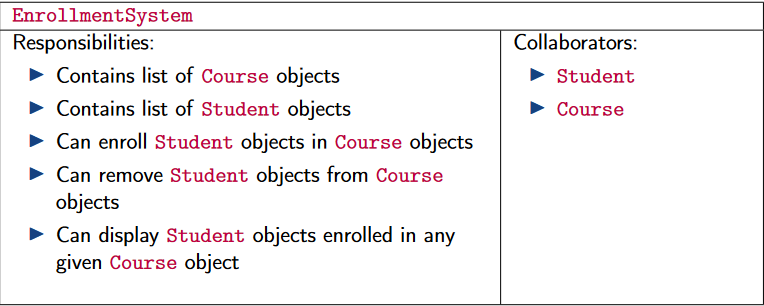
\includegraphics[width=\linewidth]{images/CRC.png}
    \end{figure}
\end{frame}

\begin{frame}{Objektorienteret Programudvikling $\Rightarrow$ Verb/noun metoden}
    \textit{Verb/noun metoden (da: udsagnsord/navneords metoden) anvendes til at identificereklasser og metoder.}
    \vspace{0.5cm}
    Ifølge verb/noun metoden er:
    \begin{itemize}
        \item \textit{Navneord kandidater} til klasser
        \item \textbf{Udsagnsord} kandidater til metoder.
    \end{itemize}
\end{frame}

\begin{frame}{Objektorienteret Programudvikling $\Rightarrow$ Verb/noun eksempel}
    \begin{figure}
        \centering
        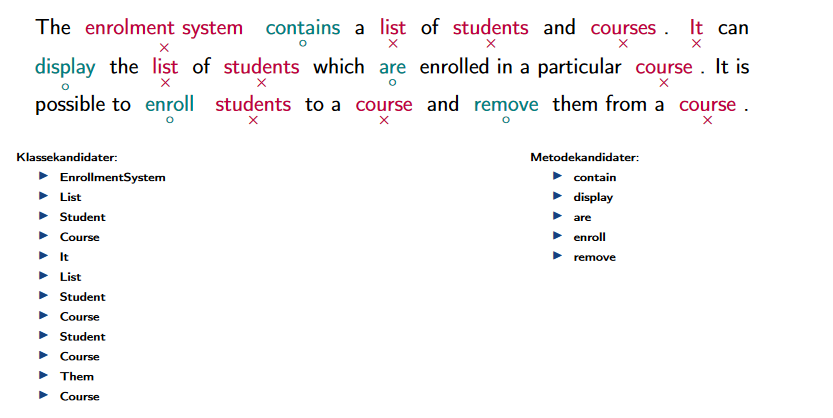
\includegraphics[width=\linewidth]{images/verb.png}
       
    \end{figure}
\end{frame}


\begin{frame}{Questions?}
            
\includegraphics[width=\linewidth, height=\paperheight]{images/man-with-question-01.png}
\end{frame}

\section{Data Strukturer}

\begin{frame}{Data Strukturer $\Rightarrow$ Contents}
    \begin{itemize}
        \item Primitive og komplekse typer
        \item Arrays
        \item Collections Frameworket
        \item List og ArrayList
        \item Map og HashMap
        \item Array, List og Map i forhold til hinanden
    \end{itemize}
\end{frame}

\begin{frame}{Data Strukturer $\Rightarrow$ Intro}
   \begin{table}[h]
\centering
\begin{tabular}{|c|c|c|}
\hline
Datatype & Possible values & Storage \\ \hline
byte & Integer: -128 to 127 & 8 bits \\ \hline
short & Integer: -32,768 to 32,767 & 16 bits \\ \hline
int & Integer: -2,147,483,648 to 2,147,483,647 & 32 bits \\ \hline
long & Integer: -9,223,372,036,854,775,808 to 9,223,372,036,854,775,807 & 64 bits \\ \hline
float & Decimal number: 7 significant digits & 32 bits \\ \hline
double & Decimal number: 15 significant digits & 64 bits \\ \hline
char & Character: A, i, ?, 2, 0, k, unicode characters*, true / false, etc. & 16 bits \\ \hline
boolean & 0 (false) or 1 (true) & 8 bits \\ \hline
\end{tabular}

\end{table}

\end{frame}


\begin{frame}[fragile]{Data Strukturer $\Rightarrow$ komplexe type}
    \textit{En kompleks type kan indeholde flere værdier.}
    \begin{itemize}
        \item Som fx. Arrays er et komplex type da den kan indeholde flere værdier:
    \end{itemize}
    \begin{lstlisting}
        int[] tobias = [1,2,3,4,5]
    \end{lstlisting}
\end{frame}

\begin{frame}[fragile]{Data Strukturer $\Rightarrow$ Arrays}
\textit{et array er en data struktur som indeholder en sekvens af andre stykker data, alle af den samme bestemte type.}
    \begin{itemize}
        \item Arrays er 0 indexerede, det vil sige at man starter ved 0 når man tæller elementer i et array.
    \end{itemize}
    \begin{lstlisting}
        String[] cars = {"Volvo", "BMW", "Ford", "Mazda"};
    \end{lstlisting}
    \begin{itemize}
        \item Her har vi et String array med bil mærke som værdier... 
    \end{itemize}
    \begin{itemize}
        \item Hvorfor bruge arrays?
        \begin{itemize}
            \item Intet behov for separate variable for associerede værdier.
            \item Evnen til let at gentage handlinger over alle elementer med loops.
            \item Antallet af elementer kan være ukendt ved programmets start.
            \begin{itemize}
                \item Hvor mange mennesker er der i et lokale?
            \end{itemize}
        \end{itemize}
    \end{itemize}
\end{frame}

\begin{frame}[fragile]{Data Strukturer $\Rightarrow$ Collection frameworket}
    \textit{Frameworket indeholder en række klasser der implementerer disse interfaces}

    Dette framework Frameworket beskriver (igennem interfaces) en række typer af datastrukturer, herunder:

    \begin{itemize}
        \item \alert{java.util.Collection} bruges til at beskrive datastrukturer der er indekserede.Altså, hvor elementer kan tilgås igennem et heltalligt indeks.
        \item \alert{java.util.Map} bruges til at beskrive datastrukturer hvor elementer kan tilgåsigennem en“nøgle”: "key $\Rightarrow$ value"
        \item \alert{java.util.Set} bruges til at beskrive mængder. Altså, hvor alle elementer er unikke
    \end{itemize}
\end{frame}

\begin{frame}[fragile]{Data Strukturer $\Rightarrow$ List og Arraylist}
    List interfacet beskriver en type af collection som er ordnet og indekserbar. Det betyder, at elementer er arrangeret i en sekvens, og at vi kan bestemme hvad derskal ligge hvor:
    \begin{itemize}
        \item boolean add (int index, T element)
        \item T remove (int index)
        \item int indexOf (T element)
    \end{itemize}
    \begin{itemize}
        \item Der er flere klasser i Java Collections Frameworket der implementerer dette interface, så som arraylists.
        \begin{itemize}
            \item En arraylist er et resizable array det vil sige at du kan slette og tilføje elementer til en arraylistem, men java documentation indeholder ikke en direkte metode til at fjerne et element fra et normal array.
        \end{itemize}
    \end{itemize}
    \begin{lstlisting}
        ArrayList<Integer> l1 = new ArrayList<Integer>();
        l1.add(0, 1);
        l1.add(1, 2);
    \end{lstlisting}
\end{frame}


\begin{frame}[fragile]{Data Strukturer $\Rightarrow$ Map og Hashmap}
    \textit{Map-interfacet definerer typer af datastrukturer, hvor værdier kan tilgås igennem 
    nøgler(eng: keys). Hvor både værdierne og nøglerne \alert{\underline{skal}} være objekter.}

    \begin{itemize}
        \item Dette svarer til en liste hvor man udpeger en værdi igennem et objekts identitet (hashCode)  i stedet for at indeksere med et heltal.
        \item Denne kode genereres via et kald til \alert{hashCode} der er defineret på \alert{Object}
    \end{itemize}

    \textit{HashMap er den oftest anvendte type af map. Med et HashMap kan man relativt hurtigt finde en placering af en value ved hjælp af en key.}

    \begin{lstlisting}
        Map<String, Person> myMap = new HashMap<>();
        Person p = new Person();
        myMap.put("Aslak", p);
        Person fromMap = myMap.get("Aslak");
    \end{lstlisting}
\end{frame}

\begin{frame}[fragile]{Data Strukturer $\Rightarrow$ Array, List og Map i forhold til hinanden}
    \begin{center}
        \begin{tabular}{|c|c|c|}
            \hline
            Array & List & Map  \\ \hline
            En klasse   & Interface  & Interface \\ 
            Elementer kan ikke slettes & Kan slettes & kan slettes \\ 
            Er ikke resizable & Resizable & Resizeable \\ 
            Har ikke key value par & Har ikke key value par & Key value par\\ \hline
        \end{tabular}
        \begin{itemize}
            \item \textit{Hvorfor er arrays en fixed størrelse?}
            \begin{itemize}
                \item Fordi at array størrelsen bliver defineret ved complie time. De er ikke er dynamiske resizable.
            \end{itemize}
        \end{itemize}
    \end{center}
    
\end{frame}


\begin{frame}{Questions?}
            
\includegraphics[width=\linewidth, height=\paperheight]{images/man-with-question-01.png}
\end{frame}


\section{Arv og Polymorfi}
\begin{frame}{Arv og Polymorfi $\Rightarrow$ Intro}
    \begin{itemize}
        \item Arv og polymorfi i kontekst af objekt-orienteret programmering
        \item Overriding
        \item Access modifiers
        \item Keywordet super
        \item Klassen Object
        \item Casting 
        \item Keywordet final
    \end{itemize}
\end{frame}


\begin{frame}{Arv og Polymorfi $\Rightarrow$ Polymorfi}
    \textit{Klasser beskriver/er skitser for objekter, der har samme struktur og adfærd.}
    \begin{itemize}
        \item “Kan det samme som klassen der arves fra, eventuelt med yderligere egenskaber”
    \end{itemize}
    \textit{Polymorfi:}
    \begin{itemize}
        \item En variabel af en given type, kan pege på objekter af denne type og alle subtyper
    \end{itemize}
\end{frame}

\begin{frame}[fragile]{Arv og Polymorfi $\Rightarrow$ Polymorfi}
    \begin{lstlisting}
        class Animal {
            public void animalSound() {
                System.out.println("The animal makes a sound");
            }
        }
        
        class Pig extends Animal {
            public void animalSound() {
                System.out.println("The pig says: wee wee");
            }
        }
        
        class Dog extends Animal {
            public void animalSound() {
                System.out.println("The dog says: bow wow");
            }
        }
    \end{lstlisting}
\end{frame}

\begin{frame}[fragile]{Arv og Polymorfi $\Rightarrow$ Arv Eksempel}
    \textit{Egenskaber (attributter og metoder) nedarves fra en klasse; ikke fra et objekt.}
    \begin{lstlisting}
        public class BaseCommand {
            String description = "Undocumented";
            
            protected boolean guardEq (String[] parameters, int bound) {
            return parameters.length!=bound;
        }
        
        public String getDescription () {
            return description;
        }
    }
    \end{lstlisting}
\end{frame}





\begin{frame}[fragile]{Arv og Polymorfi $\Rightarrow$ Arv Eksempel}
   \begin{lstlisting}
        public class CommandUnknown extends BaseCommand implements Command {
        
            @Override
            public void execute (Context context, String command, String parameters[]) {
                System.out.println("Woopsie, I don't understand '"+command+"');
            }
        }
    \end{lstlisting}
\end{frame}




\begin{frame}{Overriding $\Rightarrow$ Intro}
    \textit{Når to klasser arver den samme metode siger vi at dedeler opførsel.}
    \begin{itemize}
        \item Dette gøres ved at “override” en metode defineret i en superklasse for at definere en nyopførsel for dette metode navn.
    \end{itemize}
\end{frame}

\begin{frame}[fragile]{Overriding $\Rightarrow$ Intro}

     \begin{lstlisting}
        public interface Command {
            void execute(Context context, String command, String parameters[]);
            
            String getDescription();
        }
        
        public class CommandExit extends BaseCommand implements Command {
        
        @Override
        public void execute (Context context, String command, String parameters[]) {
            context.makeDone();
        }
    }
    \end{lstlisting}
\end{frame}

\begin{frame}{Arv og Polymorfi $\Rightarrow$ Access modifiers}
    \begin{itemize}
        \item public
        \begin{itemize}
            \item Synligt for hele projektet
        \end{itemize}
        \item private
        \begin{itemize}
            \item Kun synligt inde fra objektet/klassen
        \end{itemize}
        \item protected 
        \begin{itemize}
            \item Synligt for: klassen, packagen, og sub klasser men ikke globalt
        \end{itemize}
        \item default
        \begin{itemize}
            \item Synligt for klassen og package
        \end{itemize}
    \end{itemize}
\end{frame}

\begin{frame}[fragile]{Arv og Polymorfi $\Rightarrow$ super keywordet}
    \textit{Kan sammenlignes med \alert{this} men bruges til at tilgå elementer i en superklasse}
    \begin{lstlisting}
        public class PairOfDie {
            private int d1;
            private int d2;
            public PairOfDie(int d1, int d2){
                this.d1 = d1;
                this.d2 = d2;
            }
        }
    \end{lstlisting}
    \begin{lstlisting}
        public class GraphicalDice extends PairOfDie {
            public GraphicalDice(int d1, int d2){
                super(d1, d2);
                drawDie();
                }
            }
    \end{lstlisting}
\end{frame}


\begin{frame}{Arv og Polymorfi $\Rightarrow$ Klassen Object}
    \textit{Klassen Object er roden i klassehierarkiet. Alle klasser har Object som superklasse. Alle objekter, inklusive arrays, implementerer denne klasses metoder.}
\end{frame}

\begin{frame}[fragile]{Arv og Polymorfi $\Rightarrow$ Casting}
    \textit{Type casting er processen med at konvertere en variabel fra en datatype til en anden. I Java er der to typer af type casting: implicit og eksplicit.}

    \begin{itemize}
        \item Implicit type casting: 
        \begin{itemize}
            \item Også kendt som type promotion
            \item Automatisk konvertering af en mindre datatype til en større datatype
            \item F.eks.: En heltalsværdi tildeles en float-variabel
        \end{itemize}
        \item Eksplicit typecasting: 
        \begin{itemize}
            \item Også kendt som typekonvertering
            \item Manuel konvertering af en større datatype til en mindre datatype
            \item F.eks.: En float-værdi tildeles en heltalsvariabel
        \end{itemize}
    \end{itemize}
    \begin{lstlisting}
        int num = 10;
        float num2 = num;
    \end{lstlisting}
    \begin{lstlisting}
        float num = 10.5f;
        int num2 = (int) num;
    \end{lstlisting}
\end{frame}


\begin{frame}[fragile]{Arv og Polymorfi $\Rightarrow$ Final keywordet}
    \textit{ final er en non-access modifier, der bruges til klasser, attributter og metoder, hvilket gør dem uforanderlige (umulige at arve eller overskrive).}
    \begin{lstlisting}
        public class Main {
            final int x = 10;
            public static void main(String[] args) {
                Main myObj = new Main();
                myObj.x = 25; // will generate an error: cannot assign a value to a final variable
                System.out.println(myObj.x);
            }
        }
    \end{lstlisting}
\end{frame}

\begin{frame}{Questions?}
            
\includegraphics[width=\linewidth, height=\paperheight]{images/man-with-question-01.png}
\end{frame}


\section{Abstrakte Metoder}

\begin{frame}{Abstrakte klasser}
    \begin{itemize}
        \item Hvad er en abstrakt klasse?
        \item Hvordan anvender man abstrakte klasser?
        \item Override
        \item Interfaces
    \end{itemize}
\end{frame}

\begin{frame}{Abstrakte klasser $\Rightarrow$ Intro}
  \begin{itemize}
    \item En abstrakt klasse er en klasse som du ikke kan instansiere
    \item Abstrakte klasser kan indeholde:
    \begin{itemize}
        \item Metoder; både abstrakte og konkrete
        \item Attributter
        \item Constructorer
    \end{itemize}
  \end{itemize}
\end{frame}


\begin{frame}[fragile]{Abstrakte klasser $\Rightarrow$ Abstrakte metoder}
\begin{itemize}
    \item Erklæringen indeholder kun metode prototypen (metoden \alert{\textbf{\underline{uden}}} krop) 
    \item Abstrakte metoder \alert{\textbf{\underline{skal}}} overrides i den første konkrete subklasse i samtlige arvefølger.
\end{itemize}
\begin{verbatim}
    ⟨access modifiers⟩ abstract ⟨type⟩ (name) (⟨parameter−list⟩)
\end{verbatim}
    
\end{frame}
\begin{frame}[fragile]{Abstrakte metoder $\Rightarrow$ Anvendelse}
    \begin{lstlisting}
        abstract class Shape {
            String shape = " ";
            Shape(String n) {
                this.shape = n;
            }

            abstract double area();
            abstract double perimeter()
        }
    \end{lstlisting}
    \begin{itemize}
        \item Nu kan vi bruge disse abstrakte metoder, men vi skal nedarve fra abstrakt klassen og derefter instansiere metoderne.
    \end{itemize}
\end{frame}

\begin{frame}[fragile]{Abstrakte metoder $\Rightarrow$ Anvendelse}
     \begin{lstlisting}
        class Quadrilateral extends Shape {
            double length, width;
            Quadrilateral(double l, double w, String name) {
                super(name);
                this.l = length;
                this.w = width;
            }

            @Override
            public double perimeter() {
                return ((2*length) + (2*width));
            }

            @Override
            public double area() {
                return (length * width) 
            }
        } 
    \end{lstlisting}
\end{frame}




\begin{frame}[fragile]{Abstrakte metoder $\Rightarrow$ Anvendelse}
     \begin{lstlisting}
         class Main {
            public static void main(String[], args) {
                Shape rectangle = new Quadrilateral(3,4, "Rectangle");
                System.out.println("Area of rectangle is " + rectangle.area());
                System.out.println("Perimeter of rectangle is " + rectangle.perimeter());
            }
         }
     \end{lstlisting}
\end{frame}
\begin{frame}[fragile]{Interfaces $\Rightarrow$ Intro}
    \begin{itemize}
        \item Et interfaces definerer funktionalitet(er) som besiddes af alle klasser som implementerer det
        \item Interfaces kan ikke instantieres.

        \item Interfaces kan indeholde:
        \begin{itemize}
            \item Abstrakte metoder
            \item default
        \end{itemize}
    \end{itemize}
    \begin{verbatim}
        ⟨access modifiers⟩ interface ⟨navn⟩ {⟨krop⟩}
    \end{verbatim}
\end{frame}

\begin{frame}[fragile]{Interfaces $\Rightarrow$ Implementation}
        \begin{lstlisting}
        public interface Command {
            void execute(Context context, String command, String parameters[]);
            
            String getDescription();
        }
    \end{lstlisting}
    
\end{frame}

\begin{frame}[fragile]{Interfaces $\Rightarrow$ Implementation}
        \begin{lstlisting}
        public class CommandGo extends BaseCommand implements Command {
            public CommandGo () {
            description = "Follow an exit";
        
        @Override
        public void execute (Context context, String command, String[] parameters) {
            if (guardEq(parameters, 1)) {
                System.out.println("I don't seem to know where that is ��");
                return;
            }
            context.transition(parameters[0]);        }
}
    \end{lstlisting}
    
\end{frame}


\begin{frame}{Overriding $\Rightarrow$ Intro}
    \begin{itemize}
        \item Når to klasser arver den samme metode siger vi at dedeler opførsel.
        \item \textit{“override”} er en metode defineret i en superklasse for at definere en nyopførsel..
    \end{itemize}
\end{frame}

\begin{frame}[fragile]{Overriding $\Rightarrow$ Eksempel}
    \begin{lstlisting}
        class Parent {
            void show() { System.out.println("Parent's show()"); }
        }
 
    \end{lstlisting}
    \begin{lstlisting}
        class Child extends Parent {
            @Override 
            void show() {
                System.out.println("Child's show()");
            }
        }
    \end{lstlisting}
\end{frame}

\begin{frame}{Questions?}
            
\includegraphics[width=\linewidth, height=\paperheight]{images/man-with-question-01.png}
\end{frame}

\end{document}